\pgfplotsset{width=\linewidth, height=6cm}
\begin{figure}[h]
	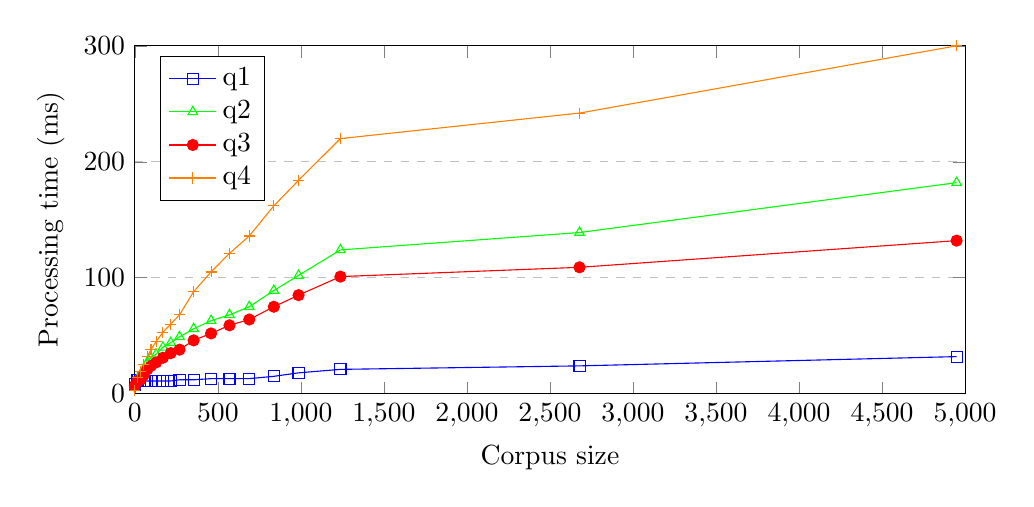
\begin{tikzpicture}[scale=1]
	\begin{axis}[
	xlabel={Corpus size},
	ylabel={Processing time (ms)},
	xmin=0, xmax=5000,
	ymin=0, ymax=300,
	legend pos=north west,
	ymajorgrids=true,
	grid style=dashed,
	%ymode=log,
	%xmode=log,
	]
	
	    \addplot[
        color=blue,
        mark=square,
        samples=100
        ]
        coordinates {
(0,8)
(16,12)
(33,11)
(53,11)
(75,11)
(97,11)
(128,11)
(169,11)
(216,11)
(269,12)
(354,12)
(459,13)
(570,13)
(689,13)
(837,15)
(986,18)
(1238,21)
(2678,24)
(4949,32)
 };

\addplot[
        color=green,
        mark=triangle,
        ]
        coordinates {
(0,7)
(16,13)
(33,16)
(53,21)
(75,27)
(97,31)
(128,34)
(169,40)
(216,44)
(269,49)
(354,56)
(459,63)
(570,68)
(689,75)
(837,89)
(986,102)
(1238,124)
(2678,139)
(4949,182)
        };

\addplot[
        color=red,
        mark=*,
        ]
        coordinates {
(0,7)
(16,11)
(33,12)
(53,16)
(75,21)
(97,24)
(128,27)
(169,31)
(216,35)
(269,38)
(354,46)
(459,52)
(570,59)
(689,64)
(837,75)
(986,85)
(1238,101)
(2678,109)
(4949,132)
        };

\addplot[
        color=orange,
        mark=+,
        ]
        coordinates {
(0,3)
(16,14)
(33,19)
(53,25)
(75,32)
(97,38)
(128,45)
(169,53)
(216,60)
(269,68)
(354,88)
(459,105)
(570,121)
(689,136)
(837,162)
(986,184)
(1238,220)
(2678,242)
(4949,300)
        };

	
	\legend{q1, q2, q3, q4}
	\end{axis}
	\end{tikzpicture}
	\caption{\label{fig:executionTime} Execution time with respect to corpus size with query expansion (ngram synonyms)}
\end{figure}